\documentclass[12pt,a4paper]{article}

% Margins.
\setlength{\oddsidemargin}{0in}
\setlength{\evensidemargin}{0in}
\setlength{\headheight}{12pt}
\setlength{\headsep}{42pt}
\setlength{\topmargin}{-54pt}
\setlength{\textwidth}{6.5in}
\setlength{\textheight}{10in}

\usepackage{amsmath}
\usepackage{float}
\usepackage{graphicx}
\usepackage[hyphens]{url}
\usepackage{hyperref}	% Clickable links to figures, references and urls.
\usepackage{datetime}
\usepackage{longtable}
\usepackage{subfigure}

% Links direct to top of figures.
\usepackage[all]{hypcap}

% Drawing.
\usepackage{pgf}
\usepackage{tikz}

% Listings for formatting code.
\usepackage{listings}
\usepackage{textcomp}
% General options.+++
\lstset{breaklines=true, basicstyle=\small\ttfamily, tabsize=4, numbers=left, stepnumber=1, frame=single, showstringspaces=false, upquote=true}
% C++ specific high-lighting. Comments are 50/50 shades of green/black and strings coloured with 60/40 red/black mixture.
\lstset{language=[ISO]C++, commentstyle=\color{green!50!black}, keywordstyle=\color{blue}, stringstyle=\color{red!60!black}}

%opening
\title{\vspace{-3cm}Physics for Engineers\\Class 34\\Magnetic Field Due to a Straight Current Carrying Wire}
\author{Attique Dawood}
\date{April 14, 2014\\[0.2cm] Last Modified: \today, \currenttime}
\begin{document}
\maketitle
\section{Announcements}
\begin{itemize}
\item Expect assignment 06 shortly.
\end{itemize}
\section{Biot--Savart Law}
Biot--Savart Law is the magnetostatics analogue of Coulomb's Law. The source of electrostatic field is a charge at rest. The source static magnetic field is a steady current (or DC current). When current flows in a wire a magnetic field is set up around the wire. The magnitude and direction of magnetic is given by the Biot--Savart Law
\begin{equation}
d\textbf{H}=\dfrac{Id\textbf{\textit{l}}\times(\textbf{r}-\textbf{r}')}{4\pi|\textbf{r}-\textbf{r}'|^{3}}.
\end{equation}
Or
\begin{equation}
d\textbf{B}=\dfrac{\mu_0Id\textbf{\textit{l}}\times(\textbf{r}-\textbf{r}')}{4\pi|\textbf{r}-\textbf{r}'|^{3}}.
\end{equation}
\section{Magnetic Field of a Current Carrying Wire}
Magnetic field due to a finite straight current carrying wire is given by
\begin{equation}
\textbf{H}=\dfrac{Ir_{12}}{4\pi|(\textbf{r}-\textbf{r}_1)\times\textbf{r}_{12}|}\left(\dfrac{(\textbf{r}-\textbf{r}_2)\cdot\textbf{r}_{12}}{|\textbf{r}-\textbf{r}_2|r_{12}}-\dfrac{(\textbf{r}-\textbf{r}_1)\cdot\textbf{r}_{12}}{|\textbf{r}-\textbf{r}_1|r_{12}}\right)\dfrac{(\textbf{r}-\textbf{r}_1)\times\textbf{r}_{12}}{|(\textbf{r}-\textbf{r}_1)\times \textbf{r}_{12}|}
\end{equation}
Here \textbf{r} is the observation point, $\textbf{r}_1$ and $\textbf{r}_2$ are end points of wire such that current is flowing from $\textbf{r}_1$ to $\textbf{r}_2$. Derivation of this equation is not a part of this course but you are expected to be able to apply and find \textbf{H} (or \textbf{B}) due to a finite straight current carrying wire.
\newpage
\section{Exercises}
\noindent\textbf{Question 1 \cite[Example 7.1, page 266]{Sadiku}:} Find \textbf{H} at (0, 0, 5) due to triangular loop shown in figure \ref{Conducting-triangular-loop}.\\
\textbf{Answer: }$\textbf{H}=\textbf{H}_1+\textbf{H}_2+\textbf{H}_3=(-59.1\hat y)+(27.4\hat x+27.4\hat y+10.9\hat z)+(-30.6\hat x+30.6\hat y)$ mA/m.
\begin{figure}[H]
\centering
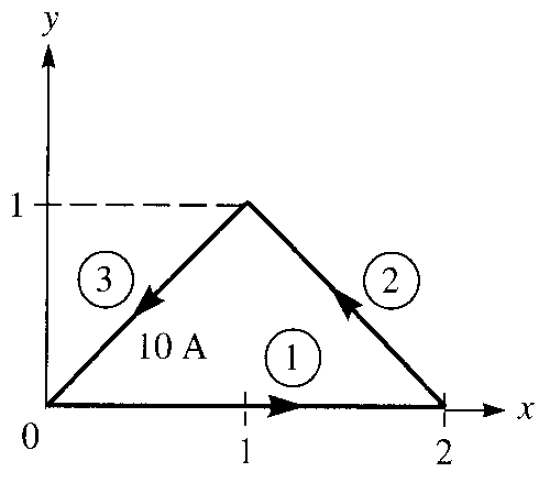
\includegraphics[scale=0.45]{Figure7-6aS.png}
\caption{Conducting triangular loop.}
\label{Conducting-triangular-loop}
\end{figure}
\noindent\textbf{Question 1 \cite[Example 7.1, page 266]{Sadiku}:} Find \textbf{H} at (-3, 4, 0) due to semi--infinite current wires shown in figure \ref{Semi-infinite-wires}.\\
\textbf{Answer: }$\textbf{H}=\textbf{H}_z+\textbf{H}_x=(38.2\hat x+28.65\hat y)+23.88\hat z$ mA/m.
\begin{figure}[H]
\centering
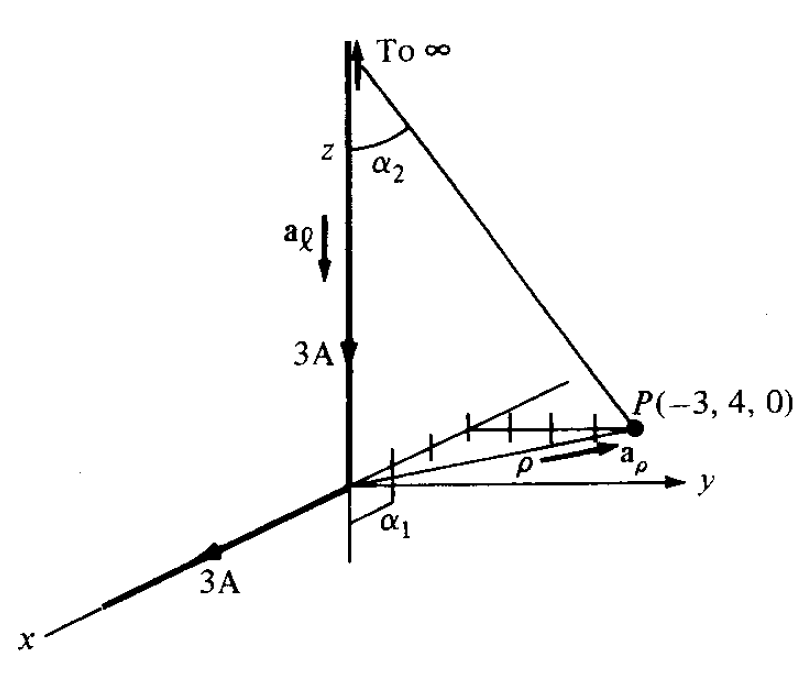
\includegraphics[scale=0.45]{Figure7-7aS.png}
\caption{Semi--infinite wires.}
\label{Semi-infinite-wires}
\end{figure}%\begin{itemize}
%\item[a.] Electric field of a point charge.
%\item[b.] Electric field of an infinite line charge placed along $z$--axis.
%\end{itemize}
%%\begin{figure}[H]
%\centering
%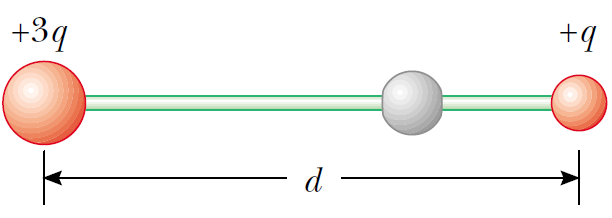
\includegraphics[scale=0.45]{FigureP23-10.png}
%\caption{Equilibrium of charge.}
%\label{Equilibrium}
%\end{figure}
%\nocite{*}
\bibliographystyle{plain}
\bibliography{PhysicsRef}
\end{document}
